\hspace{24pt}
In this section, first we introduce dataset and some tools, then we will explain the steps of our experiment, and then analyze the experimental results in three different simulation scenarios, and finally use the VCF file from dbSNP and divide it into SNP and INDEL according to the type of mutation Discuss the experimental results separately.

\section{Dataset}
Eagle needs three main input files, they are reference genome (FASTA), read data (FASTQ), and variant file (VCF). 

First, the reference genome sequencing data is Genome Reference Consortium Human Build 37 patch release 13 (GRCh37.p13) version from NCBI website. There are 1 to 22, X and Y chromosome of primary assembly and some extra sequences.

Second, the read sequencing data is real sequencing data from NA12878 which is a cell line of an individual female from a CEPH pedigree that is Utah residents with Northern and Western European ancestry, using an exome sequencing dataset (Garvan HG001) by sequencer HiSeq2500 from Genome-In-A-Bottle (GIAB).

Third, we will use VCF files from the Single Nucleotide Polymorphism Database (dbSNP). dbSNP is a public domain archive for a wide collection of simple genetic polymorphisms. The polymorphism set includes single bases. Base nucleotide substitutions (also called single nucleotide polymorphisms or SNPs) , small-scale multi-base deletions or insertions (also called deletion insertion polymorphisms or INDELs), We will discuss according to these two different types.

Last, Finally, we will also use the simulated VCF file, the variant file is generated by our simulation, we provide more details on the next chapter.

\section{Simulation workflow}
In order to carefully evaluate our effect and verify whether our method can reduce the influence of reference bias, we use simulation methods to conduct experiments. We modify the GRCh37 reference genome sequence to simulate the actual occurrence of mutations in our reference genome (Figure\ref{f4-1}), record the result of our modification to generate simulate VCF file.

\vspace{1cm}
\begin{figure}[H]
    \centering
    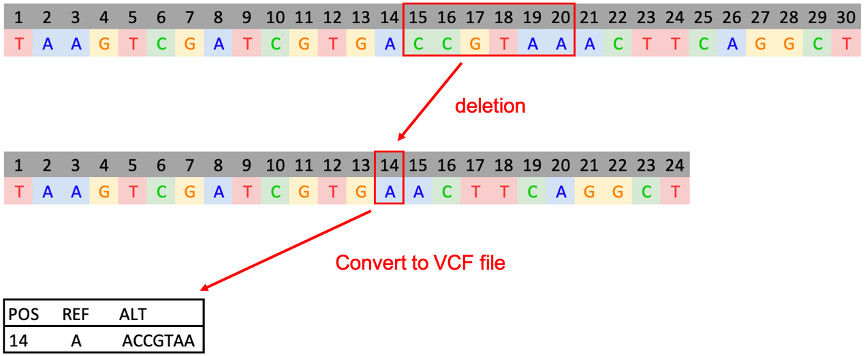
\includegraphics[width=1\columnwidth]{body/image/4-1.png}
    \captionsetup{labelfont=bf}
    \renewcommand{\baselinestretch}{1.0}
    \vspace{-1cm}
    \caption[Simulate variants]{Simulate variants.}
    \label{f4-1}
\end{figure}

Then we will use BWA, follow the traditional approach, and do the alignment again. Use the re-alignment step to simulate the occurrence of reference bias, because we modified the reference, when re-alignment, the pileup at the original position will have some reads affected by the reference bias, and these affected reads will be misalignment or incorrect alignments. After generating the files needed by eagle, we can start our experiment, and the whole experiment process will look like Figure \ref{f4-2}.

\vspace{1cm}
\begin{figure}[H]
    \centering
    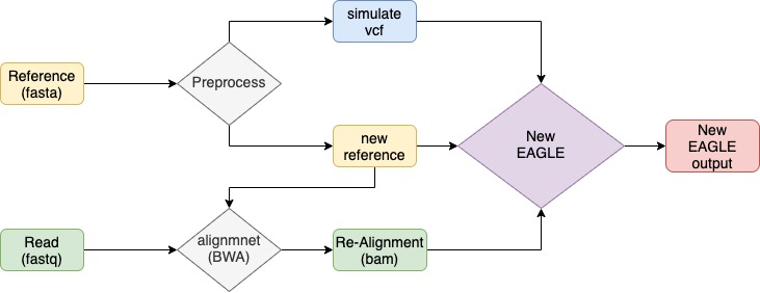
\includegraphics[width=1\columnwidth]{body/image/4-2.png}
    \captionsetup{labelfont=bf}
    \renewcommand{\baselinestretch}{1.0}
    \vspace{-1cm}
    \caption[Simulation workflow]{Simulation workflow.}
    \label{f4-2}
\end{figure}

In addition, we use SAMtools to check the pile-up read depth, and test it in 3 cases according to different pile-up read depth(Table \ref{t4-1}), discussing different pile-up read depth, we reduce the influence of reference bias

\vspace{0.5cm}
\begin{table}[h]
    \centering
    \caption[total indels amount]{total simulate indels amount}
    \vspace{-0.5cm}
    \begin{tabular}{c}
        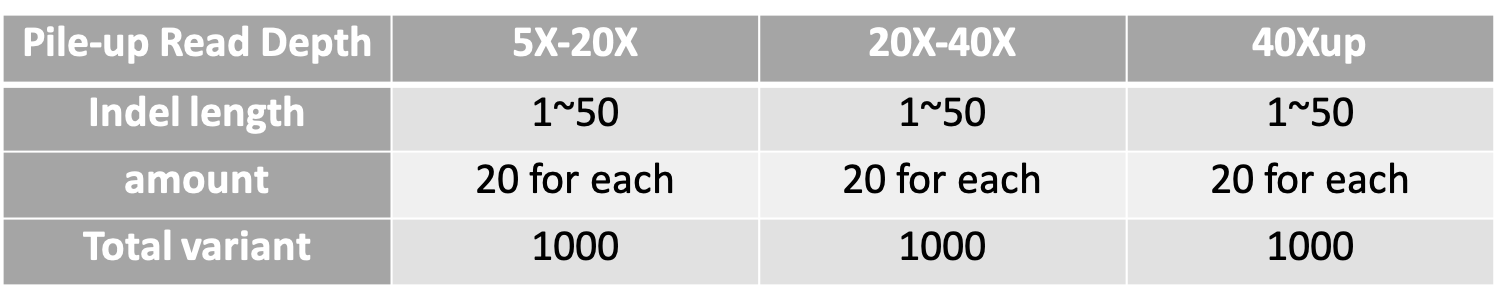
\includegraphics[width=1\textwidth]{body/image/t4-1.png}
    \end{tabular}
    \label{t4-1}
\end{table}

For each case, we will simulate 20 variants for indels of different lengths from 1 to 50. At the same time, we will discuss the results after re-alignment into two situations, one is that after re-alignment, BWA can still find read and generate pileup at that position, and the other is that after re-alignment, no read can be aligned to that position.

For the first case, EAGLE is still able to evaluate the variants, so the focus of our discussion will be the changes in EAGLE evaluation after the introduction of our method. For the second case, we will focus on the results calculated by EAGLE
\begin{flushleft}
And our evaluation standard is to observe the output of eagle for each variant odds:  
\end{flushleft}
\begin{center}
    log⁡(P[Alt|v]/P[Ref|v])
\end{center}

\section{Case 1: Low pile-up read depth}

First of all, we can see that for the original eagle found (Table \ref{t4-2} the first two rows), We can see that in the case of low pile-up read depth, since we only have a small number of reads, once there is a reference bias, we will easily be severely affected. And therefore most of our reads cannot be aligned correctly to the right position, at the same time, you can also see that the longer the length of indels, the more serious the impact, but relatively, after we find the read, it also has more impact on the longer indels.

\vspace{1cm}
\begin{table}[h]
    \centering
    \caption[low pile-up read depth variants]{low pile-up read depth variants}
    \vspace{-0.5cm}
    \begin{tabular}{c}
        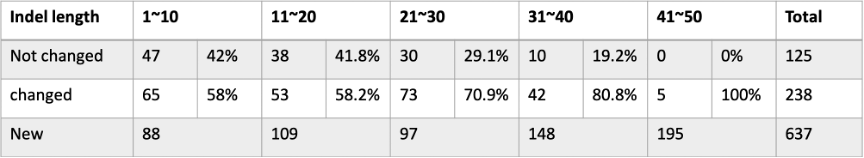
\includegraphics[width=1\textwidth]{body/image/t4-2.png}
    \end{tabular}
    \label{t4-2}
    %\tabfnt
    {Note: Explain that in the case of low pile-up read depth, after we add read, eagle evaluates the number of variants affected.}
\end{table}

Next, let’s take a look at the changes after adding our method. We can see that eagle prefers that the position does not contain variants in the original judgment, but in most cases (82\%), when we find some reads that contain variants, we can help eagle judge whether the position contains variants. (Table \ref{t4-3})

\vspace{1cm}
\begin{center}
\begin{table}[h]
    \centering
    \caption[Changes in the number of variants with lower pile-up read depth]{Changes in the number of variants with lower pile-up read depth}
    \vspace{-0.5cm}
    \begin{tabular}{c}
        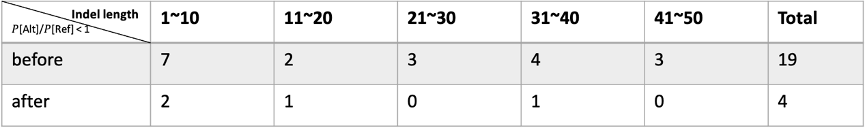
\includegraphics[width=1\textwidth]{body/image/t4-3.png}
    \end{tabular}
    \label{t4-3}
\end{table}
\end{center}

We checked the cases that changed after we found the read, and we found that most of the examples were as we predicted, and we were able to find reads in FASTQ that were misalignment due to reference bias. Figure \ref{f4-3} is one of the cases.

\vspace{1cm}
\begin{figure}[H]
    \centering
    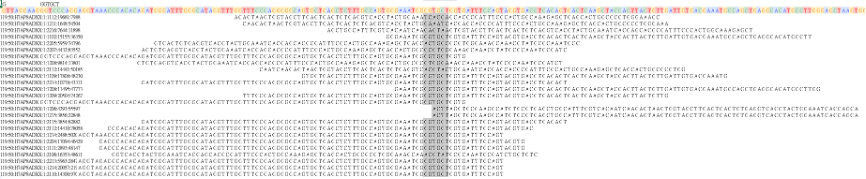
\includegraphics[width=1\columnwidth]{body/image/4-3.png}
    \captionsetup{labelfont=bf}
    \renewcommand{\baselinestretch}{1.0}
    \vspace{-1cm}
    \caption[New reads in a region with low pile-up read depth]{Example of new reads supporting a variant in a region with low pile-up read depth.}
    \label{f4-3}
\end{figure}

Similarly, there are some reads that we find more ref biased. This is because when we change reference sequence, we don't require the base of each position to be the same as the reference genome, so this situation is reasonable. (Figure \ref{f4-4})

\vspace{1cm}
\begin{figure}[H]
    \centering
    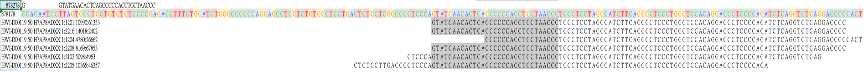
\includegraphics[width=1\columnwidth]{body/image/4-4.png}
    \captionsetup{labelfont=bf}
    \renewcommand{\baselinestretch}{1.0}
    \vspace{-1cm}
    \caption[New reads are similar to the reference with low pile-up read depth]{Example where new reads found are also similar to the reference sequence with low pile-up read depth.  Note repetitive nature of the surrounding genome sequence.}
    \label{f4-4}
\end{figure}

Next, we can look at the comparison of eagle odds. 
The numerical calculation method is:
odd(after)/odd(before)
, can represent our help to EAGLE

\vspace{1cm}
\begin{figure}[H]
    \centering
    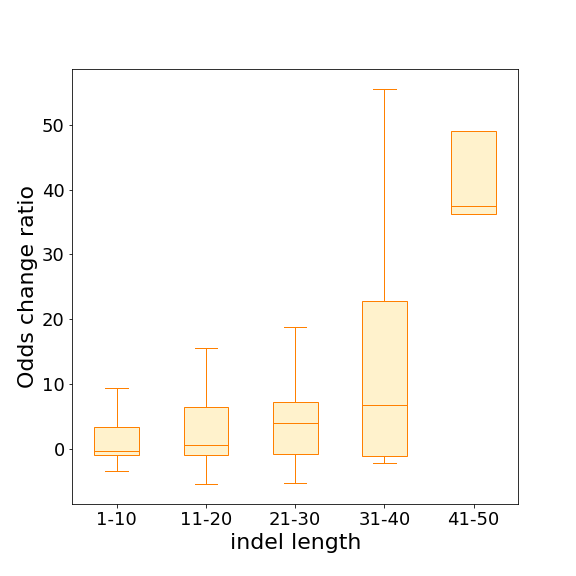
\includegraphics[width=0.6\columnwidth]{body/image/4-5.png}
    \captionsetup{labelfont=bf}
    \renewcommand{\baselinestretch}{1.0}
    \caption[low pile-up read depth odds change ratio]{The vertical axis shows the change in EAGLE log odds ratio of variant to reference for indel variants, grouped by length (horizontal axis).  Change here meaning the difference in the log odds ratio when when using the read index versus only using the pile-up.  Plotted for variants from low pile-up read depth regions.}
    \label{f4-5}
\end{figure}

In the case of low pile-up read depth, first of all, we can observe that after we add read, the confidence value of most of the variants increases because we find more reads that contain mutations (Figure \ref{f4-5}), and regardless of the length of the indel, their distribution of odds increase percentage is mostly above zero.
This may mean that even in the case of low pile-up read depth, our method is very helpful for most mutation points, especially for indels with a length of 40 or more, where the increase is particularly obvious.

Finally, we look at the last row of Table \ref{t4-2}, we can see these positions are affected by the reference bias, so that no read can be mapped to these positions to form a pileup. Our method is obviously very helpful. For the remaining variants in the 1,000 variants, we can find those reads that are affected by reference bias and are lost, thereby helping eagle evaluate the possibility of these mutations.

\vspace{0.5cm}
\begin{figure}[H]
    \centering
    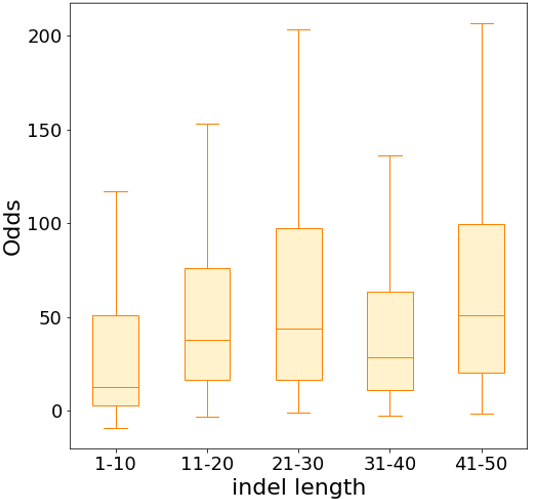
\includegraphics[width=0.6\columnwidth]{body/image/4-6.png}
    \captionsetup{labelfont=bf}
    \renewcommand{\baselinestretch}{1.0}
    \caption[no reads with variants from low pile-up depth odds ratio]{The vertical axis shows the EAGLE log odds ratio of variant to reference for indel variants, grouped by length (horizontal axis).  Plotted for variants occurring in regions with no reads from low pile-up depth.}
    \label{f4-6}
\end{figure}

Then see the odds calculated by eagle after we find the read (Figure \ref{f4-6}), we can see the odds calculated by eagle. For most of the variants, eagle gives the conclusion that contained the variant at this position, which is also in line with our expected results.


\section{Case 2: Medium pile-up read depth}
\begin{center}
\begin{table}[h]
    \centering
    \caption[medium pile-up read depth variants]{medium pile-up read depth variants}
    \vspace{-0.5cm}
    \begin{tabular}{c}
        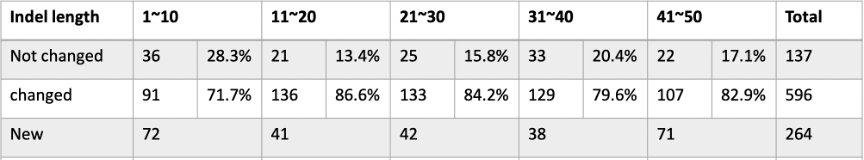
\includegraphics[width=1\textwidth]{body/image/t4-4.png}
    \end{tabular}
    \label{t4-4}
    %\tabfnt
    {Note: Explain that in the case of medium pile-up read depth, after we add read, eagle evaluates the number of variants affected.}
\end{table}
\end{center}

First of all, we can see that in this case,Table \ref{t4-4}, because of the increase in pile-up read depth, the variants affected by reference bias are significantly reduced, and the number of reads that we can overlap with the variant position has also increased. For the same reason, more misaligned reads are affected by reference bias.

\vspace{1cm}
\begin{table}[h]
    \centering
    \caption[Changes in the number of variants with medium pile-up read depth]{Changes in the number of variants with medium pile-up read depth}
    \vspace{-0.5cm}
    \begin{tabular}{c}
        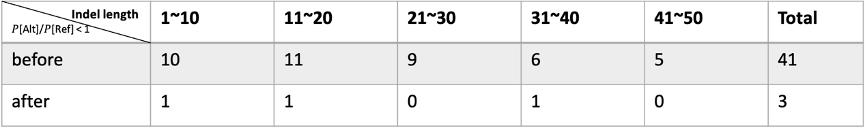
\includegraphics[width=1\textwidth]{body/image/t4-5.png}
    \end{tabular}
    \label{t4-5}
\end{table}

With the same increase in pile-up read depth, In EAGLE’s initial judgment, the number of tendencies that position does not contain variant has also increased, because more misalignments have occurred. And just for this reason, the more reads that we can find to help EAGLE. Therefore, we can see that after we find the read, the affected variant has also increased, nearly 91\% of vaiants in Table \ref{t4-5} have been changed to the correct situation. (Figure \ref{f4-7} ,\ref{f4-8} are some examples)

\vspace{1cm}
\begin{figure}[H]
    \centering
    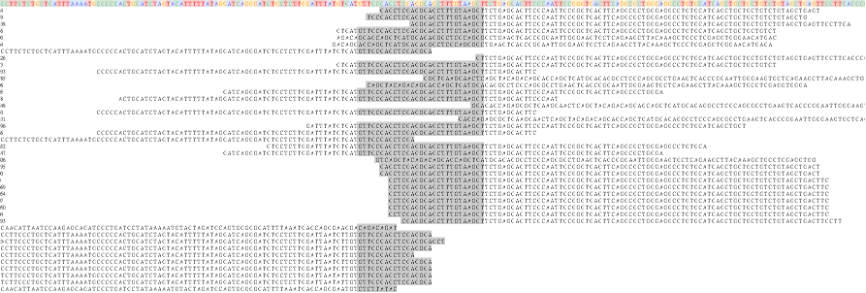
\includegraphics[width=1\columnwidth]{body/image/4-7.png}
    \captionsetup{labelfont=bf}
    \renewcommand{\baselinestretch}{1.0}
    \vspace{-1cm}
    \caption[New reads in a region with medium pile-up read depth]{Example of new reads supporting a variant in a region with medium pile-up read depth.}
    \label{f4-7}
\end{figure}

\begin{figure}[H]
    \centering
    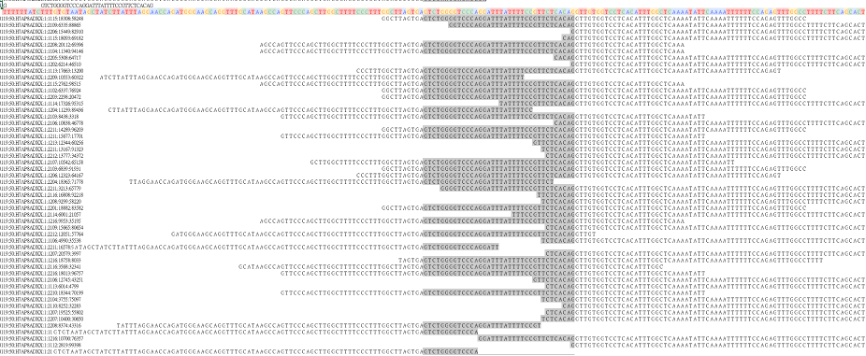
\includegraphics[width=1\columnwidth]{body/image/4-8.png}
    \captionsetup{labelfont=bf}
    \renewcommand{\baselinestretch}{1.0}
    \vspace{-1cm}
    \caption[New reads are similar to the reference with medium pile-up read depth]{Example where new reads found are also similar to the reference sequence with medium pile-up read depth.  Note repetitive nature of the surrounding genome sequence.}
    \label{f4-8}
\end{figure}

We can find that in bad cases, although we found reads similar to hypothetical sequences, we did not improve the score of EAGLE on variants. In these few examples, we found that their mutated sequences happened to be repeated sequences. Therefore, the similarity between it and the reference sequence is also very high(Figure \ref{f4-9}). We think facing this reason squarely affects EAGLE's judgment on him

\vspace{1cm}
\begin{figure}[H]
    \centering
    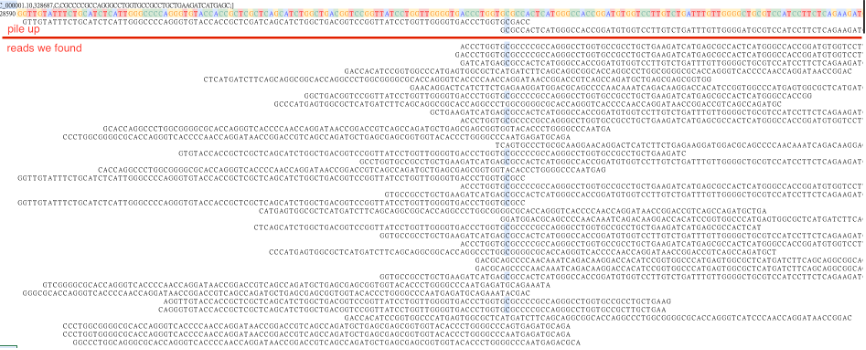
\includegraphics[width=1\columnwidth]{body/image/4-9.png}
    \captionsetup{labelfont=bf}
    \renewcommand{\baselinestretch}{1.0}
    \vspace{-1cm}
    \caption[pileup with Figure \ref{f4-8}]{pileup with Figure \ref{f4-8}.}
    \label{f4-9}
\end{figure}


\begin{figure}[H]
    \centering
    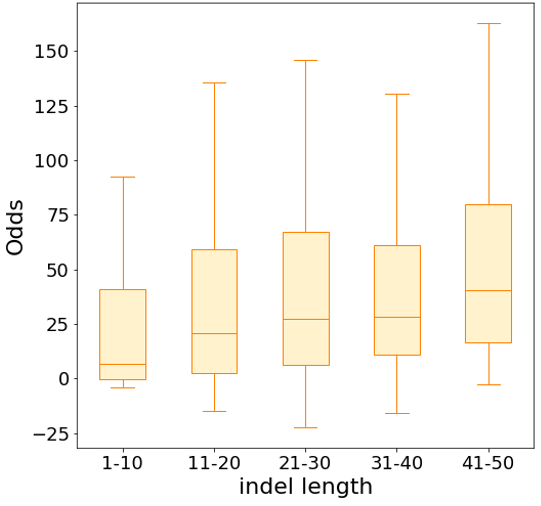
\includegraphics[width=0.6\columnwidth]{body/image/4-10.png}
    \captionsetup{labelfont=bf}
    \renewcommand{\baselinestretch}{1.0}
    \caption[medium pile-up read depth odds change ratio]{The vertical axis shows the change in EAGLE log odds ratio of variant to reference for indel variants, grouped by length (horizontal axis).  Change here meaning the difference in the log odds ratio when when using the read index versus only using the pile-up.  Plotted for variants from medium pile-up read depth regions.}
    \label{f4-10}
\end{figure}

Next, we can look at the comparison of eagle odds in medium pile-up read depth (Figure \ref{f4-10}). Basically, the change is similar to the situation of low pile-up read depth. We can also see larger growth in the longer indel. The difference is that we also have a good performance in the shorter indel. And the average growth rate is better than that of low pile-up read depth. This result is quite reasonable, because we find more reads that match the variant, which can help eagle give these mutations greater confidence.
We can also see that indels with a length of 10 or more on our boxplot have Q3 greater than 0, which means that most of our reads can help us eliminate the influence of reference bias.

\vspace{0.5cm}
\begin{figure}[H]
    \centering
    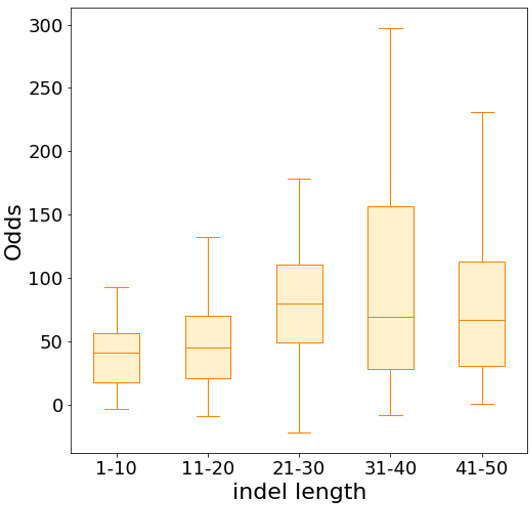
\includegraphics[width=0.6\columnwidth]{body/image/4-11.png}
    \captionsetup{labelfont=bf}
    \renewcommand{\baselinestretch}{1.0}
    \caption[no reads with variants from medium pile-up depth odds ratio]{The vertical axis shows the EAGLE log odds ratio of variant to reference for indel variants, grouped by length (horizontal axis).  Plotted for variants occuring in regions with no reads from medium pile-up depth.}
    \label{f4-11}
\end{figure}


Finally, we look at the last row of Table 4-4, we can see that our method still can help some variants that EAGLE cannot calculate because there is no pileup at the position. Figure \ref{f4-11} shows these variant odds calculated by eagle.

In this case, EAGLE can get more correct conclusions, that is, the position does contain variants, because we can find more read support variants. It can be seen that compared to the previous case, regardless of the length of the indel, their Q3 is 0 some distance higher, this result is also as we predicted ,and Figure \ref{f4-12} is some example.

\vspace{1cm}
\begin{figure}[H]
    \centering
    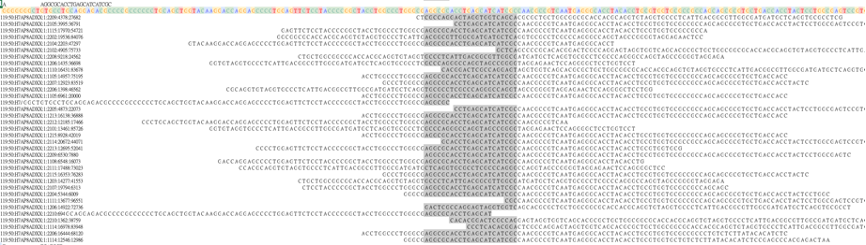
\includegraphics[width=1\columnwidth]{body/image/4-12.png}
    \captionsetup{labelfont=bf}
    \renewcommand{\baselinestretch}{1.0}
    \vspace{-1cm}
    \caption[find new pileup reads in medium pile-up read depth]{find reads on no pileup position.}
    \label{f4-12}
\end{figure}

\section{Case 3: High pile-up read depth}
\begin{table}[h]
    \centering
    \caption[high pile-up read depth variants]{high pile-up read depth variants}
     \vspace{-0.5cm}
    \begin{tabular}{c}
        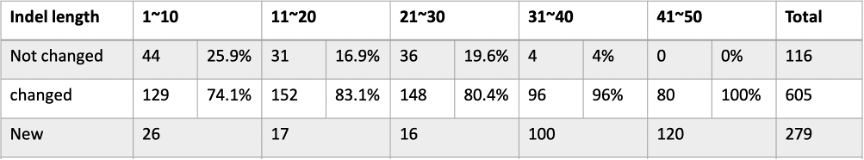
\includegraphics[width=1\textwidth]{body/image/t4-6.png}
    \end{tabular}
    \label{t4-6}
    %\tabfnt
    {Note: Explain that in the case of high pile-up read depth, after we add read, eagle evaluates the number of variants affected.}
\end{table}


Basically, in this case, we will observe results that are very similar to medium pile-up read depth, that's because there are quite a lot of reads, most positions can still produce pileup (Table \ref{t4-6}).

\vspace{1cm}
\begin{table}[h]
    \centering
    \caption[Changes in the number of variants with high pile-up read depth]{Changes in the number of variants with high pile-up read depth}
    \vspace{-0.5cm}
    \begin{tabular}{c}
        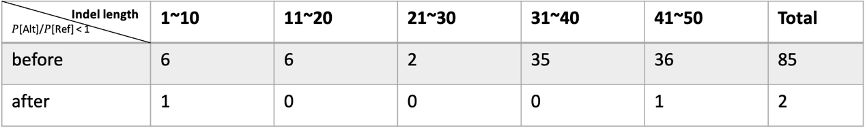
\includegraphics[width=1\textwidth]{body/image/t4-7.png}
    \end{tabular}
    \label{t4-7}
\end{table}

Interestingly, here we observe that the pile-up read depth rate is twice as high as that of the medium pile-up read depth, EAGLE initially judged that the position does not contain variation, but also through our method, we can complete more corrections than the medium pile-up read depth case. There are nearly 97\% of variants in Table \ref{t4-7} have been changed to the correct situation. (Fig \ref{f4-13},\ref{f4-14} are some examples)

\vspace{1cm}
\begin{figure}[H]
    \centering
    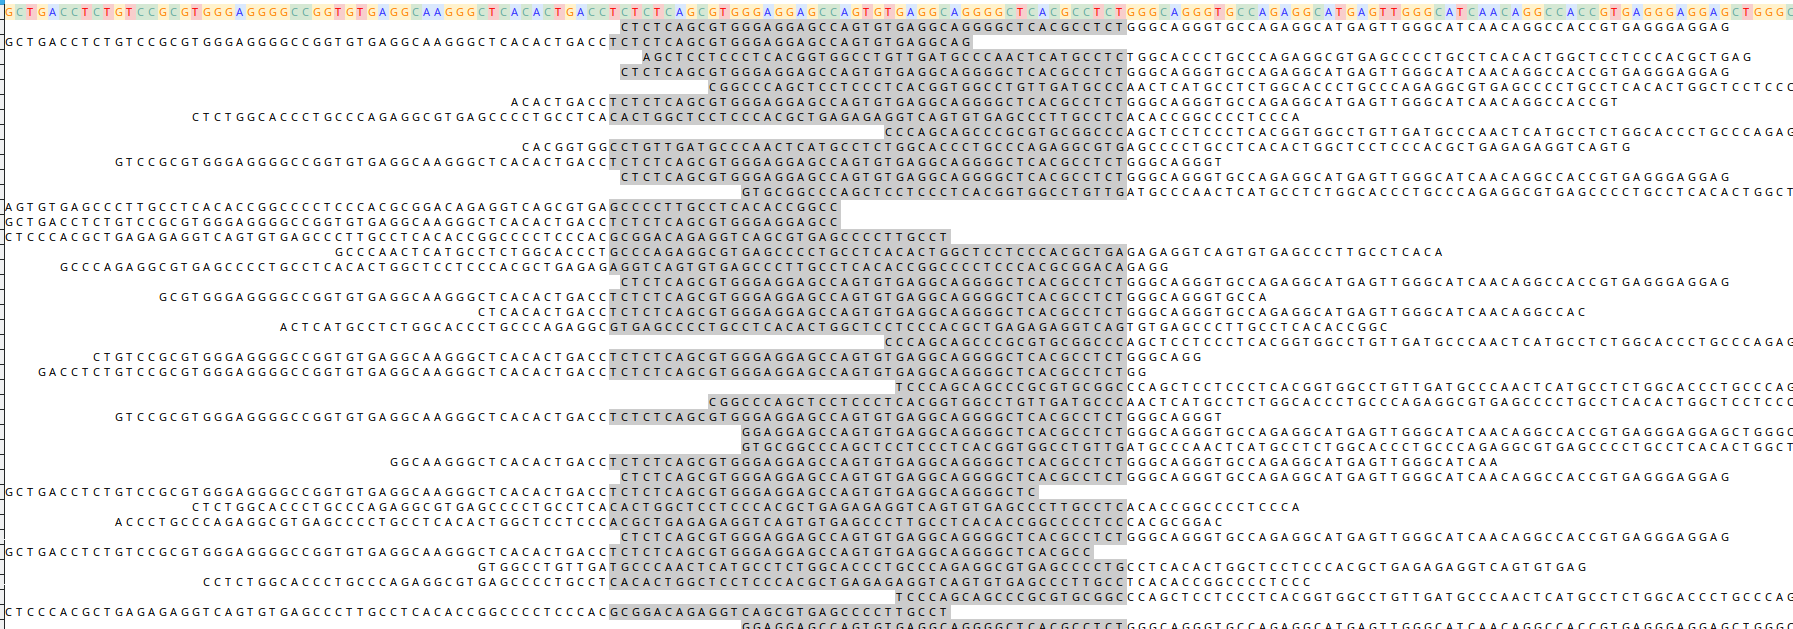
\includegraphics[width=1\columnwidth]{body/image/4-13.png}
    \captionsetup{labelfont=bf}
    \renewcommand{\baselinestretch}{1.0}
    \vspace{-1cm}
    \caption[New reads in a region with high pile-up read depth]{Example of find large amount new reads supporting a variant in a region with high pile-up read depth.}
    \label{f4-13}
\end{figure}
\vspace{0.5cm}
\begin{figure}[H]
    \centering
    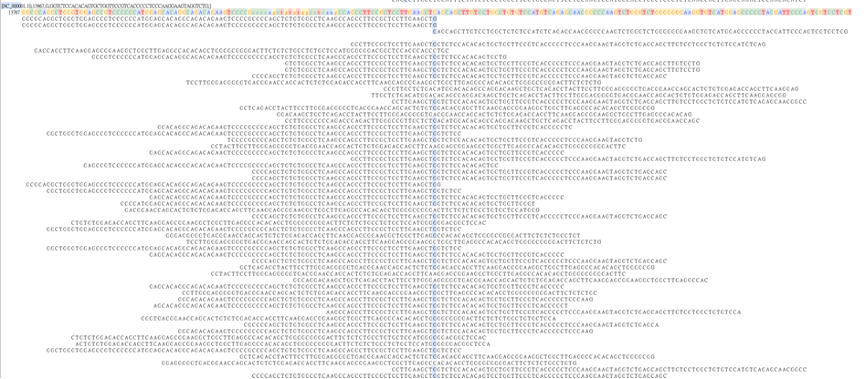
\includegraphics[width=1\columnwidth]{body/image/4-14.png}
    \captionsetup{labelfont=bf}
    \renewcommand{\baselinestretch}{1.0}
    \vspace{-1cm}
    \caption[variant pileup in high pile-up read depth]{Pileup after adding reads.}
    \label{f4-14}
\end{figure}

Then, we look at the comparison of eagle odds in high pile-up read depth (Figure \ref{f4-15}). It can be seen that compared with the previous example, it is very obvious that the longer the indel, the better the growth. However, we found many cases where the length of the mutation is greater than 50. This also shows that the more reads that we can find that are lost, the better we can reduce the impact of reference bias.

\begin{figure}[H]
    \centering
    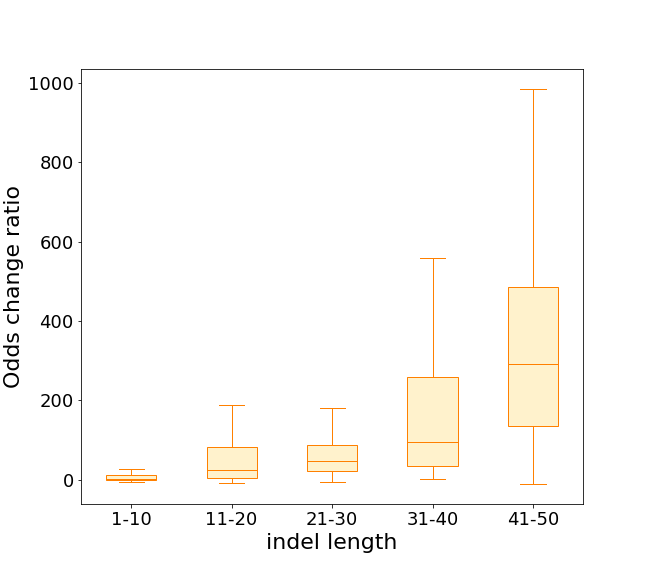
\includegraphics[width=0.6\columnwidth]{body/image/4-15.png}
    \captionsetup{labelfont=bf}
    \renewcommand{\baselinestretch}{1.0}
    \caption[high pile-up read depth odds change ratio]{The vertical axis shows the change in EAGLE log odds ratio of variant to reference for indel variants, grouped by length (horizontal axis).  Change here meaning the difference in the log odds ratio when when using the read index versus only using the pile-up.  Plotted for variants from high pile-up read depth regions.}
    \label{f4-15}
\end{figure}

Finally, we look at the last row of Table 4-6, we can see the same result as the previous case medium pile-up read depth. Figure 4-16 shows these variant odds calculated by eagle.

\begin{figure}[H]
    \centering
    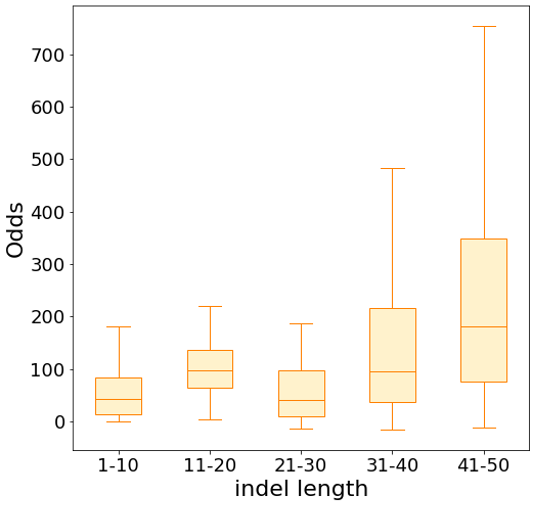
\includegraphics[width=0.6\columnwidth]{body/image/4-16.png}
    \captionsetup{labelfont=bf}
    \renewcommand{\baselinestretch}{1.0}
    \caption[no reads with variants from high pile-up depth odds ratio]{The vertical axis shows the EAGLE log odds ratio of variant to reference for indel variants, grouped by length (horizontal axis).  Plotted for variants occuring in regions with no reads from high pile-up depth.}
    \label{f4-16}
\end{figure}


\section{SNPs in dbSNP dataset}

There are 15,936,832 SNP variants form the dpSNP dataset, we random select 100,000 variants from the dataset, and the amount of matching pileup of the querying SNP variants are 50488. After joining our method, there are 22995 variants that have been changed as a result, we have looked at a few cases (Figure \ref{f4-17},\ref{f4-18},\ref{f4-19},\ref{f4-20}), we find many sequences that include the variants.

\vspace{0.5cm}
\begin{figure}[H]
    \centering
    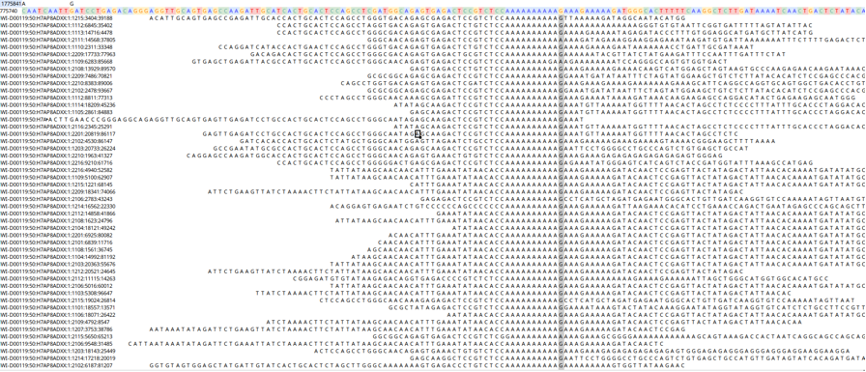
\includegraphics[width=1\columnwidth]{body/image/4-17.png}
    \captionsetup{labelfont=bf}
    \renewcommand{\baselinestretch}{1.0}
    \vspace{-1cm}
    \caption[SNP match reads]{ found match reads with hypothetical sequence in SNP.}
    \label{f4-17}
\end{figure}

\vspace{0.5cm}
\begin{figure}[H]
    \centering
    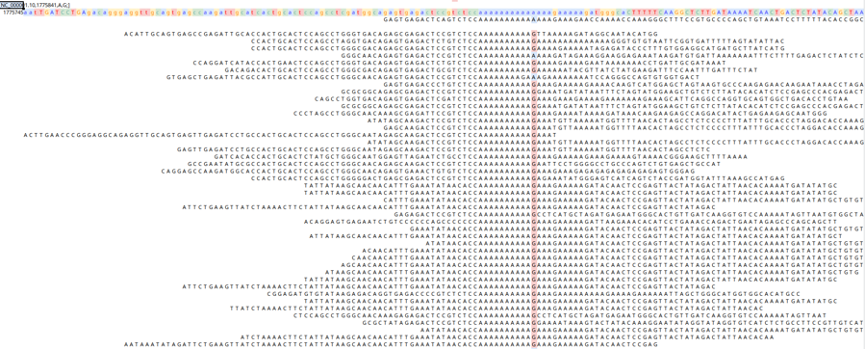
\includegraphics[width=1\columnwidth]{body/image/4-18.png}
    \captionsetup{labelfont=bf}
    \renewcommand{\baselinestretch}{1.0}
    \vspace{-1cm}
    \caption[Figure 4.17 pileup]{ The pileup corresponding to the Figure 4-17 variants.}
    \label{f4-18}
\end{figure}

\begin{figure}[H]
    \centering
    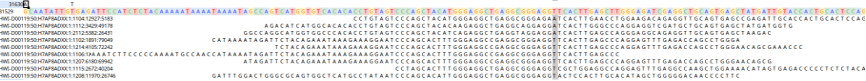
\includegraphics[width=1\columnwidth]{body/image/4-19.png}
    \captionsetup{labelfont=bf}
    \renewcommand{\baselinestretch}{1.0}
    \vspace{-1cm}
    \caption[SNP worse match reads]{ found match reads but more similar to reference sequence in SNP.}
    \label{f4-19}
\end{figure}

\vspace{0.5cm}
\begin{figure}[H]
    \centering
    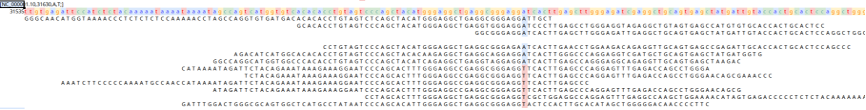
\includegraphics[width=1\columnwidth]{body/image/4-20.png}
    \captionsetup{labelfont=bf}
    \renewcommand{\baselinestretch}{1.0}
    \vspace{-1cm}
    \caption[Figure 4.19 pileup]{The pileup corresponding to the Figure 4-19 variants.}
    \label{f4-20}
\end{figure}

And we can find that the read we found gives eagle more basis for judgment, but the magnitude of the change is not very obvious in the SNPs (Figure 4-21), and most of them are less than 0. We speculate that the single-base nucleotide substitutions will not have a great impact on the alignment results.

\vspace{1cm}
\begin{figure}[H]
    \centering
    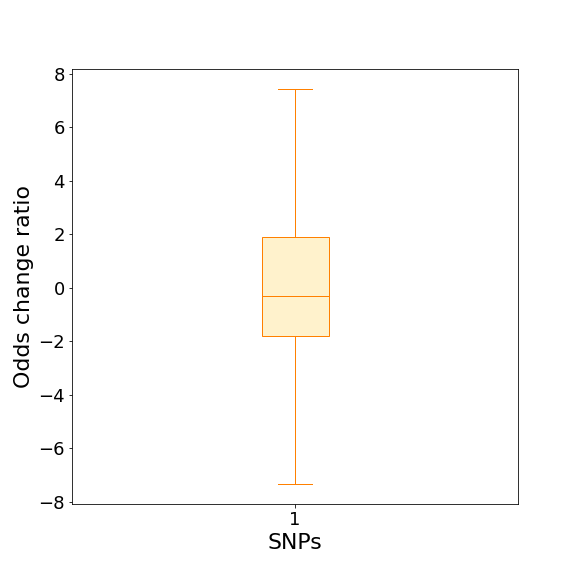
\includegraphics[width=0.6\columnwidth]{body/image/4-21.png}
    \captionsetup{labelfont=bf}
    \renewcommand{\baselinestretch}{1.0}
    \caption[SNPs odds change ratio]{SNPs odds change ratio.}
    \label{f4-21}
\end{figure}

\section{INDELs in dbSNP dataset}

There are 1,759,193 INDEL variants form the dpSNP dataset, we random select 10,000 variants from the dataset, and the amount of matching pileup of the querying INDEL variants are 5093. After joining our method, there are 2482 variants that have been changed as a result, we have looked at a few cases  (Figure \ref{f4-22},\ref{f4-23},\ref{f4-24},\ref{f4-25}).

\vspace{1cm}
\begin{figure}[H]
    \centering
    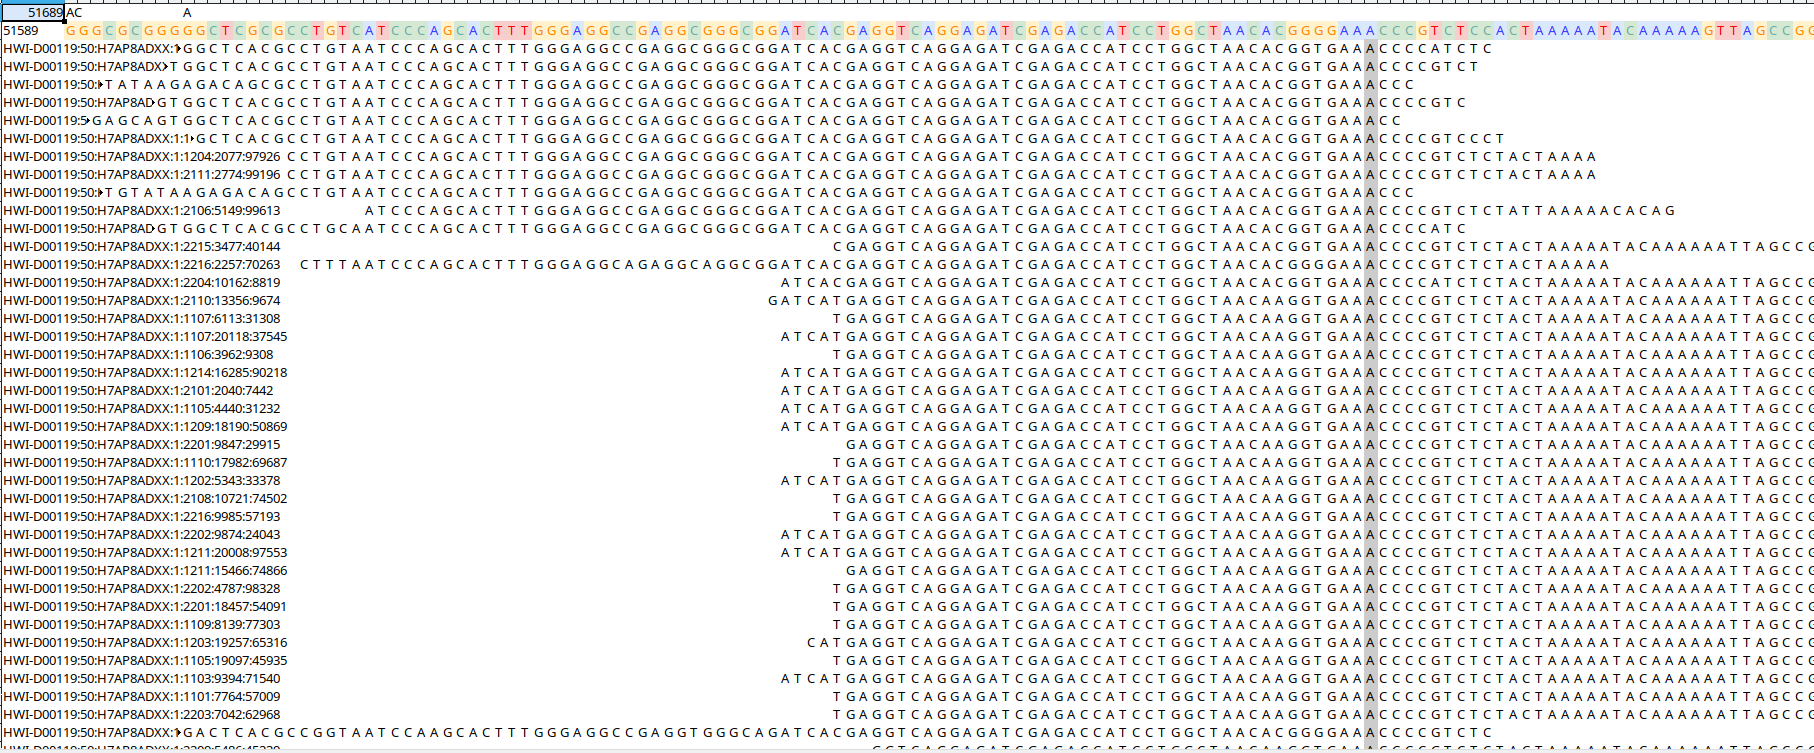
\includegraphics[width=1\columnwidth]{body/image/4-22.png}
    \captionsetup{labelfont=bf}
    \renewcommand{\baselinestretch}{1.0}
    \vspace{-1cm}
    \caption[INDEL match reads]{ found match reads with hypothetical sequence in INDEL.}
    \label{f4-22}
\end{figure}

\vspace{0.5cm}
\begin{figure}[H]
    \centering
    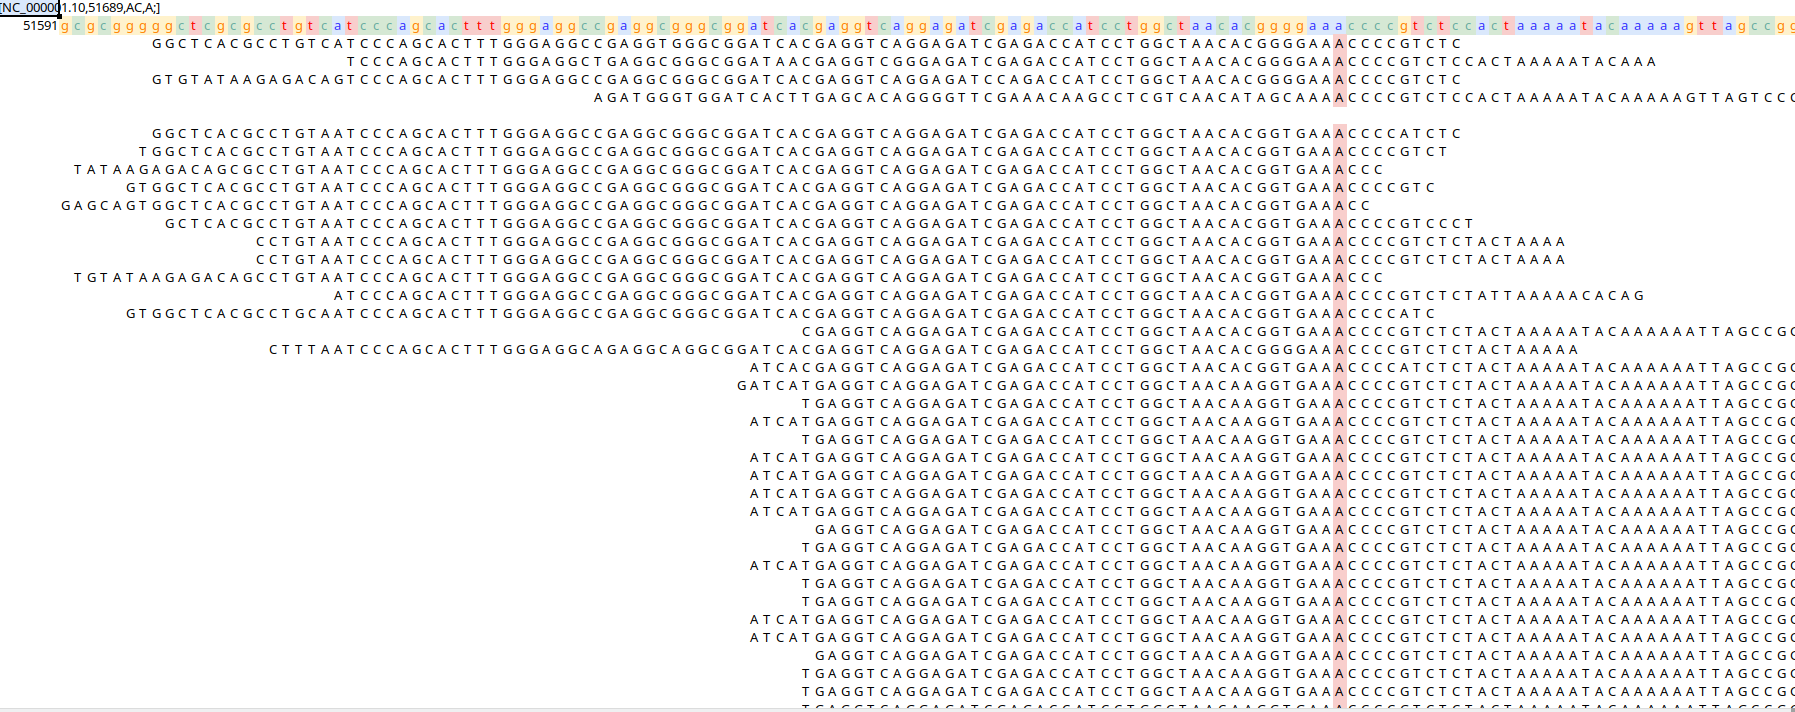
\includegraphics[width=1\columnwidth]{body/image/4-23.png}
    \captionsetup{labelfont=bf}
    \renewcommand{\baselinestretch}{1.0}
    \vspace{-1cm}
    \caption[Figure 4.22 pileup]{ The pileup corresponding to the Figure 4-22 variants.}
    \label{f4-23}
\end{figure}

\begin{figure}[H]
    \centering
    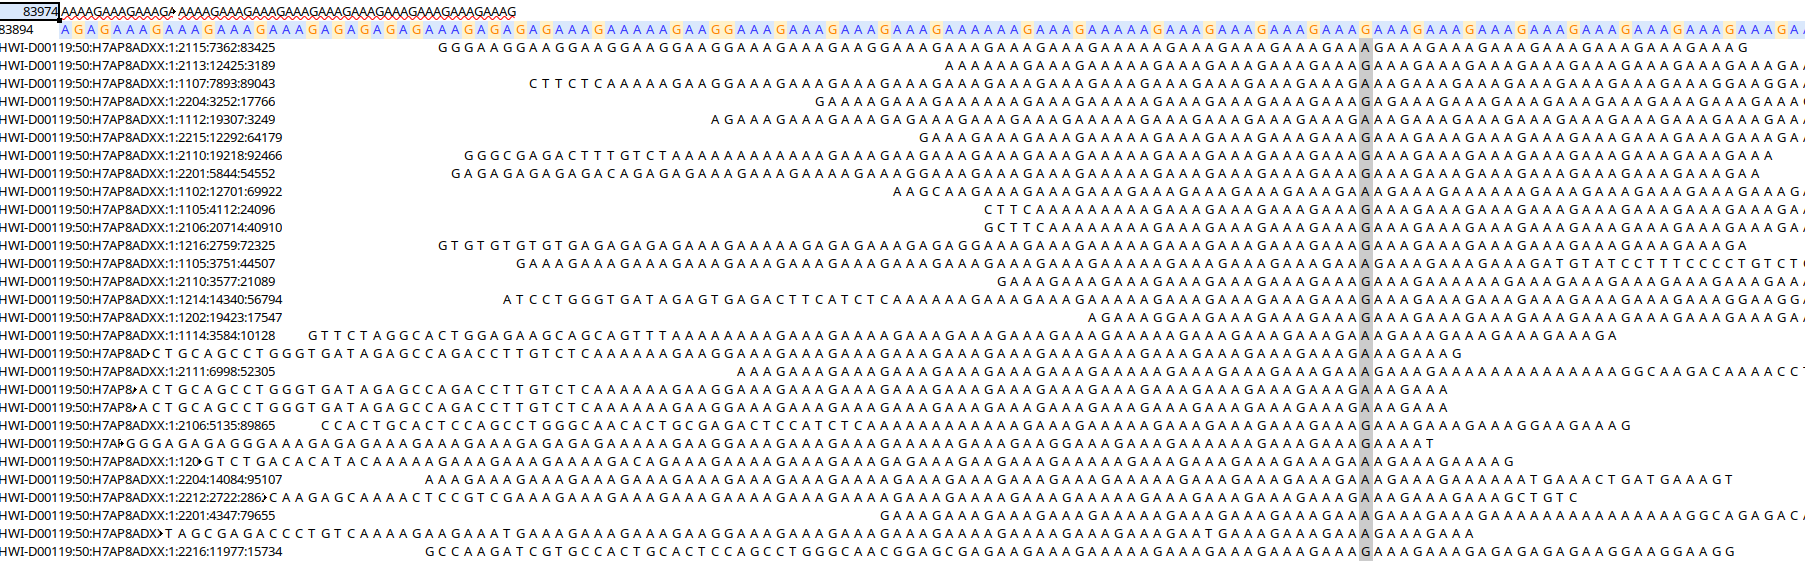
\includegraphics[width=1\columnwidth]{body/image/4-24.png}
    \captionsetup{labelfont=bf}
    \renewcommand{\baselinestretch}{1.0}
    \vspace{-1cm}
    \caption[INDEL worse match reads]{ found match reads but more similar to reference sequence in INDEL.}
    \label{f4-24}
\end{figure}

\vspace{0.5cm}
\begin{figure}[H]
    \centering
    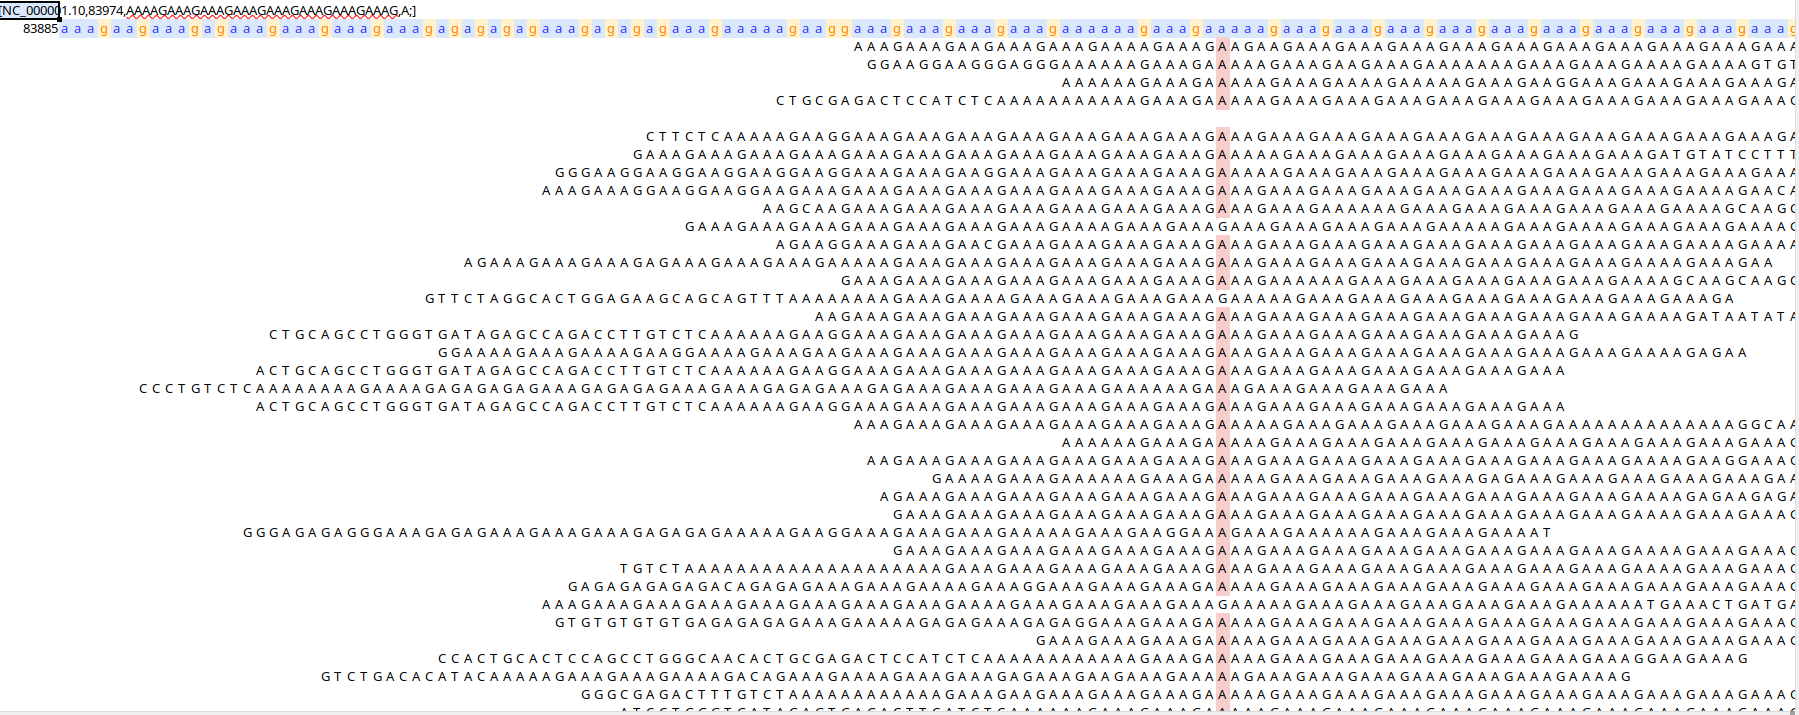
\includegraphics[width=1\columnwidth]{body/image/4-25.png}
    \captionsetup{labelfont=bf}
    \renewcommand{\baselinestretch}{1.0}
    \vspace{-1cm}
    \caption[Figure 4.24 pileup]{The pileup corresponding to the Figure 4-24 variants.}
    \label{f4-25}
\end{figure}

It can also be found that the read we found gave eagle more evidence for judgment, but the magnitude of change in INDEL was significantly greater than SNP, just like the experiment we simulated before.

\begin{figure}[H]
    \centering
    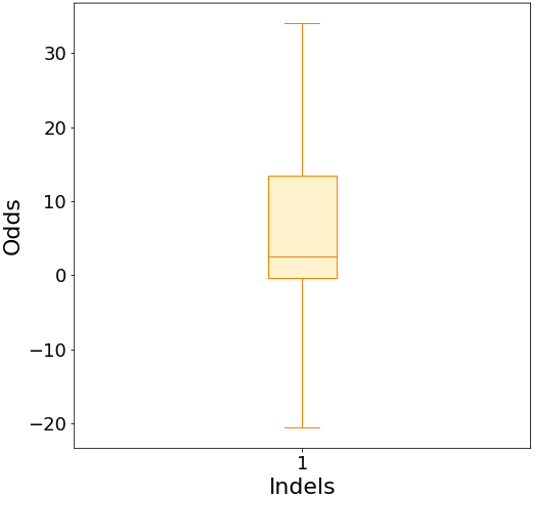
\includegraphics[width=0.6\columnwidth]{body/image/4-26.png}
    \captionsetup{labelfont=bf}
    \renewcommand{\baselinestretch}{1.0}
    \caption[INDEL odds change ratio]{INDEL odds change ratio.}
    \label{f4-26}
\end{figure}

\section{Execution time and memory consumption}

Finally, let’s discuss our execution time and memory consumption, our test data are as follows Table\ref{t4-8}, test environment as Figure \ref{f4-27}.

\vspace{1cm}
\begin{table}[h]
    \centering
    \caption[Test Dataset]{Test Dataset}
    \vspace{-0.5cm}
    \begin{tabular}{c}
        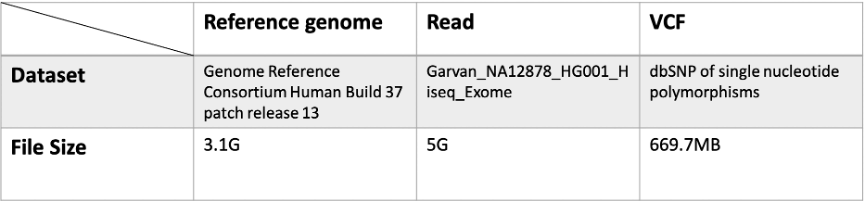
\includegraphics[width=1\textwidth]{body/image/t4-8.png}
    \end{tabular}
    \label{t4-8}
\end{table}

\begin{figure}[H]
    \centering
    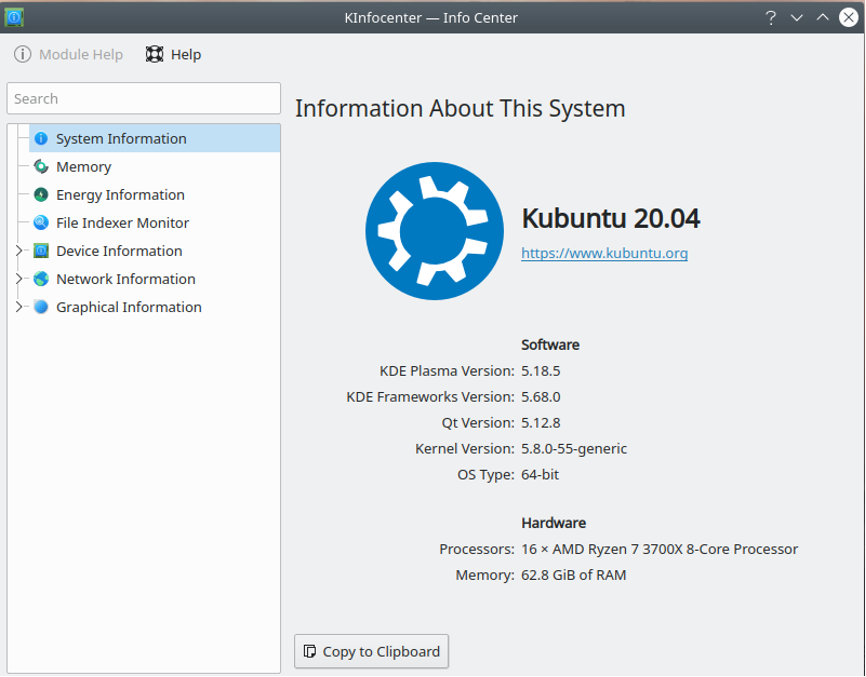
\includegraphics[width=0.8\columnwidth]{body/image/4-27.png}
    \captionsetup{labelfont=bf}
    \renewcommand{\baselinestretch}{1.0}
    \caption[Test Environment]{Test Environment.}
    \label{f4-27}
\end{figure}

Experimenting with the above conditions, first we can see that the memory we consume is 11.64G, and the memory consumed by EAGLE is 0.36G, we can find that the memory space we need is indeed much larger than the original EAGLE. This is because we need to access read-index, reference-index and read files to complete quick searches, so the memory size we need is closely related to these three.
But what we care most about is our execution speed. The time taken by EAGLE is 3618.18 seconds and our method is 6426.28 seconds. Although it seems to take a lot of time, we can find out that we have increased by carefully analyzing our execution time. A large part of the time is to index the read. The time it takes is 1649.33 seconds, and the time we search is very quick, as shown in Figure \ref{f4-28}, and a part of the time is because we find more reads, the calculation added by EAGLE Time. Considering this situation, we can say that the added time is relatively small.

\begin{figure}[H]
    \centering
    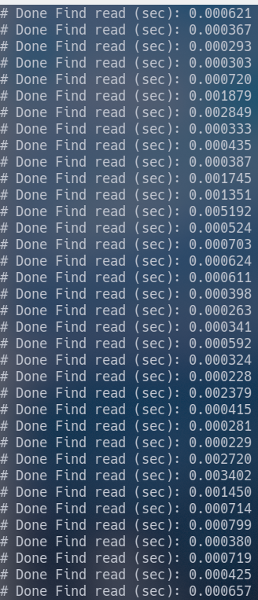
\includegraphics[width=0.4\columnwidth]{body/image/4-28.png}
    \captionsetup{labelfont=bf}
    \renewcommand{\baselinestretch}{1.0}
    \caption[searching time]{searching per hypothetical sequence time.}
    \label{f4-28}
\end{figure}
